\section{Experimental setup.}
The CLAS spectometer is divided in six sectors, each with a $\theta$ coverage
up to $140^0$.
Each sector contains the following detectors (as shown in Fig. \ref{fig:clas}):
\begin{itemize}
\item Three regions of drift chambers (DC).
\item A \v Cerenkov detector (CC).
\item Time of flight scintillators (TOF).
\item An electromagnetic calorimeter (EC).
\end{itemize}
Region two of the DC is inside a torodoial magnetic field produced
by superconducting coils, which extend from region one to three. The system of coils is called {\it torus }
(also visible in Fig.  \ref{fig:clas} in yellow).
Two sectors (one and two) are also covered by a large angle calorimeter with coverage up to $90^0$ (LAC).
Inside region one of the drift chamber another toroidal magnetic field is produced by a {\it minitorus}
to bend m\o eller electrons towards the beam dump away from the detectors.
\begin{figure}[h] 
 \begin{center}
  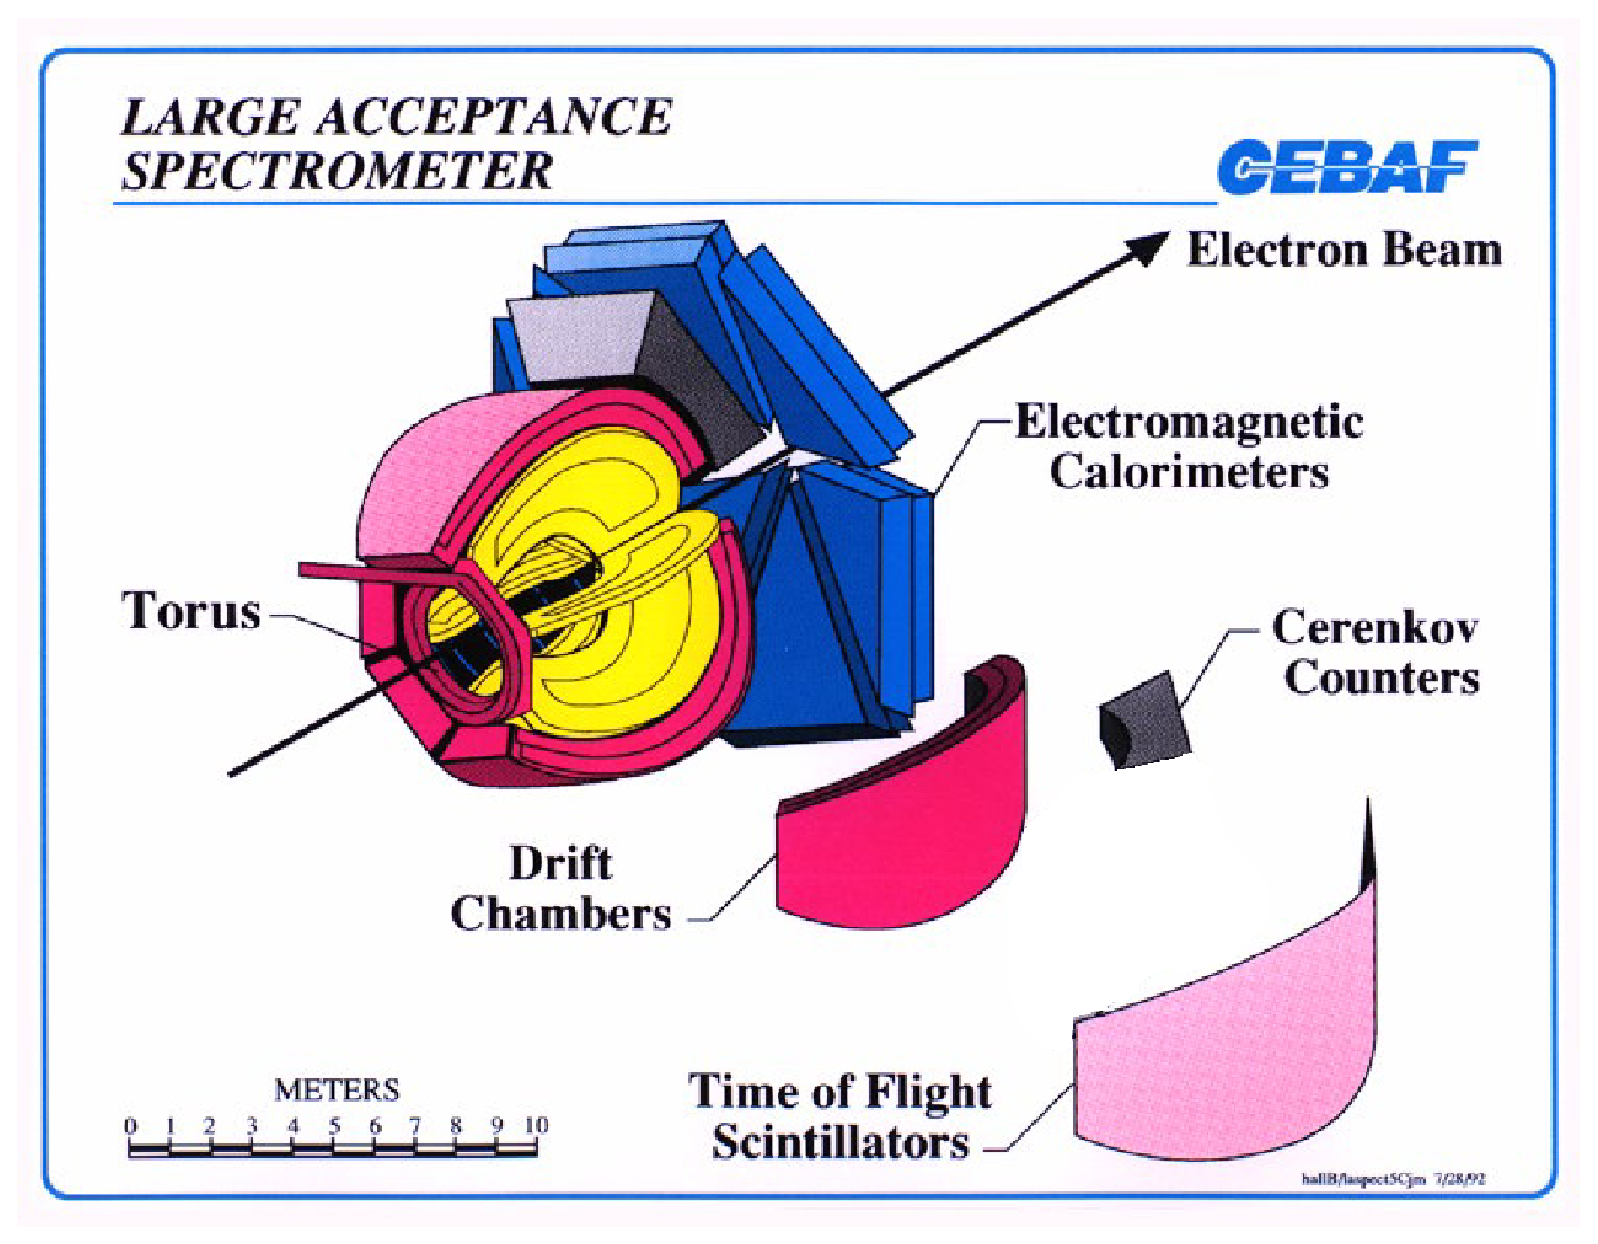
\includegraphics[width=10cm]{img/clas.eps} 
  \caption{\cit Structure of CLAS.  Only DC region 3 (red) is explicitly labeled, along with
               Time of flight (pink), \v Cerenkov (grey) and EC detectors (blue). 
               Torus coils are also shown (in yellow).}
  \label{fig:clas}
 \end{center}
\end{figure}
The data under this analysis come from the so called {\bf e16} running period.

\subsection{Run conditions for e16.}
This set of data was taken from October 2001 to January 2002 with the following conditions:
\begin{itemize}
\item Beam energy: 5.754 GeV
\item Full torus magnetic field (3375A) to bend negative tracks toward beam line.
\item Full minitorus magnetic field (6000A) to prevent m\o eller electrons from going into CLAS detector.
\item Trigger: coincidence of hits in forward calorimeter (EC) and \v Cerenkov detector
\item Current intensity: ~5 nA, which corresponds to a luminosity of $7\times 10^{33}cm^{-2}s^{-1}$ 
\item Number of triggers: ~ 3.7 billion.
\end{itemize} 
